\chapter{Implementation}
\label{cha:implementation}

\section{Costumer}
The costumer role refer to any individual who send a package through the system.
as discussed in the design paragraph the costumer has the following features:

\begin{description}[font=$\bullet$~\normalfont\scshape\color{red!50!black}]
\item register a package
\item delete a package with status "registered"
\item show a package detail view 
\item time line
\end{description}

\subsection{Register a package}
The register package process divided by two component:
\begin{description}[font=$\bullet$~\normalfont\scshape\color{red!50!black}]
\item RegisterPackage.js - view (child)
\item UserSpace.js - controller (father)
\end{description}


\begin{figure}[!ht]
	\centering
	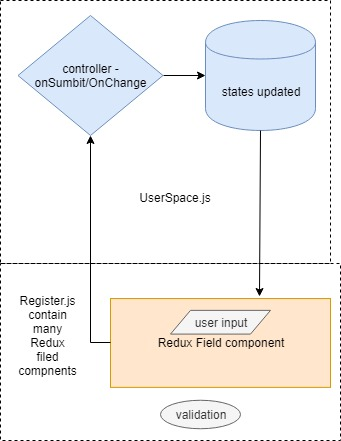
\includegraphics[width=0.5\textwidth]{images/register.jpg}
	\caption{register package process, component diagram}
	\label{fig:}
\end{figure}


The component ResgiterPackage is an assembly of Redux <Field> component.
for each input field the user enter the form get render and the state is updated
The form contain the following validation:
\begin{description}[font=$\bullet$~\normalfont\scshape\color{red!50!black}]
\item no text input filed can be left empty 
\item receiver mail must be a register user
\end{description}
i.e with out full filling the constrains the user can not press the submit button

